%***********************************************%
%												%
% EECS 470 - Lab 01 Assignment					%
%<------------------> 							%
% Last Modified by:								%
%	William Cunningham on 2014-9-03				%
%												%
%***********************************************%

%***********************************************%
% Preamble										%
%***********************************************%

\documentclass[dvipsnames]{article}

\usepackage{xcolor}
\usepackage[os=win]{menukeys}

\usepackage{
	tikz,
	colortbl,
	graphicx,
	amsmath,
	amssymb,
	mathrsfs,
	hyperref,
	float,
	siunitx,
	fancyhdr,
	url,
	minted,
	cleveref
}

\usepackage
	[left=1in,top=1in,right=1in,bottom=1in]
	{geometry}

\pagestyle{fancy}

%--- Header ---%

\newcommand{\courseNumber}{EECS 470}
\newcommand{\courseTitle}{Computer Architecture}
\newcommand{\university}{University of Michigan, Ann Arbor}
\newcommand{\labdate}{Monday, January 17$^\text{th}$, 2021}


\lhead{
	\small{
		\university
	}
}
\rhead{
	\small{
		\emph{Date: \labdate} \hspace*{-1em}
		% Why is the above \hspace necessary?
	}
}

\newcommand{\shortbar}{
	\vspace*{-12pt}
	\begin{center}
		\rule{5ex}{0.1pt}
	\end{center}
}
\newcommand{\lab}[1]{
	\begin{center}
		\LARGE{
			\vspace*{-32pt}
			EECS 470 Lab #1 Assignment
			\shortbar
			\vspace*{-20pt}
		}
	\end{center}
}


%***********************************************%
%                                               %
% TikZ Definitions                              %
%                                               %
%***********************************************%
\usetikzlibrary{shapes,arrows,automata,shadows}
\pgfdeclarelayer{background}
\pgfdeclarelayer{foreground}
\pgfsetlayers{background,main,foreground}

% Block Diagram Styles
\tikzstyle{block} = [draw, fill=RoyalBlue!50, rectangle,
        minimum height=2cm, minimum width=2cm, rounded corners]
\tikzstyle{sum} = [draw, fill=blue!20, circle, node distance=2cm]
\tikzstyle{input} = [coordinate]
\tikzstyle{output} = [coordinate]
\tikzstyle{branch} = [coordinate]
\tikzstyle{pinstyle} = [pin edge={to-, thin, black}]

% Signal Flow Graph Styles
\tikzstyle{state} = [draw, fill=RoyalBlue!50, circle,
	minimum height=3em]

%***********************************************%
%                                               %
% Document										%
%                                               %
%***********************************************%

\begin{document}
\lab{1}

\section*{Note:}
\begin{itemize}
	\item Please review the \href{https://caenfaq.engin.umich.edu/linux-login/how-do-i-connect-to-a-caen-linux-computer-remotely}{\underline{CAEN VNC help page}} to get setup for the rest of this lab.	
	\item Please review the \href{https://docs.google.com/document/d/1U9FOOYAPqvhSQda-v66SCmUgdvuaBs1KIK8Ht4_WSCA/edit?usp=sharing}{\underline{GTKwave Waveform Viewer tutorial}} as a fallback option instead of DVE. The tutorial below explains how to use DVE. DVE is a more powerful tool but is often very slow when used remotely.
	\item The lab should be completed individually. 
	\item The lab must be checked off by a GSI before end of lab on Friday,
		January 29$^\text{th}$, 2021.
	\begin{itemize}
		\item It is \texttt{highly} recommended you complete the lab before the following week's lab release
		\end{itemize}
\end{itemize}

\section{Linux Introduction and Setup}
The work in this class will be done using tools installed in the CAEN Linux
environment. You will need to log in to Linux if you haven't already done so.
Once you are logged in, you will need to open a terminal; right click on the
desktop and select ``open terminal'' from the list that pops up. 

There are a number of useful things that you can do in the terminal besides
running the tools associated with this class. Here is a short introduction to a
few of the most useful items.

\subsection{File System Utilities}
The file system that your home directory is stored in is an Andrew File System
(AFS) cell. To interact with this, you run the command \texttt{fs}. There are
many useful subcommands, including setting file permissions (\texttt{fs
setacls}) and checking your space allocation (\texttt{fs quota}). The latter is
quite important because the tools used in this class can use up your entire
space allocation if you're not careful. This tutorial is unlikely to do so, but
the final project very well might.

\subsection{Text Editors}
CAEN supplies a number of text editors. It is beyond the scope of this tutorial
and this class to proselytize for one over the other, but we do recommend that
you get familiar with at least one terminal-based text editor, which generally
means \texttt{vim}, \texttt{emacs} or \texttt{nano}. Graphical text editors
available include SublimeText2 and Gedit. 

\subsection{Bourne Again Shell (\texttt{bash})}
We will discuss the shell in much greater depth in lab 5, but you might want to
do some reading on your own.

\subsection{Setup}
This tutorial has a set of starter files, which you need to download from the course web site under ``Schedule".

% The
% easiest way is to use the \texttt{wget} tool, which goes something like:

% \noindent 
% \texttt{\$ wget www.eecs.umich.edu/courses/eecs470/labs/lab1.tar.gz}

\noindent
Once you have the tarball, you need to extract it:

\noindent
\texttt{\$ tar -xvf lab1.tar.gz}

\noindent
Now that you have the files, it's time to get started on the tutorial. 
\section{Synopsys Tools}
\subsection{The Build System: GNU Make}
Due to the complexity of the Synopsys tools, we are using the GNU Make build
system to compile and run simulations. You will need to get familiar with this,
particularly for the final project. We will be giving you a much more thorough
introduction next week in lab. 

For most of your assignments before the final project, you will simply be able
to reuse the Makefile we provide with this lab without much, if any,
modification. You will be required to reuse the standard naming conventions in
this \texttt{Makefile}.

\begin{figure}[H]
	\inputminted[frame=lines,obeytabs,tabsize=4,firstline=15,lastline=15]{makefile}{Makefile}
	\inputminted[frame=lines,obeytabs,tabsize=4,firstline=25,lastline=27]{makefile}{Makefile}
	\caption{Makefile variables}
	\label{fig:makevar}
\end{figure}

We will now walk through the provided Makefile to help you understand the
basics. \Cref{fig:makevar} shows the way that Make handles variables. The
declaration of the \texttt{VCS} variable is pretty standard. Here, we use that
variable to hold the command for compiling the simulator for your design. You
will not need to modify this variable, but you will need to modify the variables
for the design files. 


\begin{itemize}
	\item \texttt{TESTBENCH} - this variable holds the name of your testbench 
		file
	\item \texttt{SIMFILES} - this variable holds the names of all the
		synthesizable Verilog files you are working with
	\item \texttt{SYNFILES} - this variable holds the names of all the 
		synthesized Verilog files, which are generated by the synthesis tool and
		typically end in \texttt{*.vg}.
\end{itemize}

After the variables are declared, the rest of the file is dedicated to Make 
rules. These rules are the components that allow Make to do dependency
resolution. You may want to add a few, particularly related to synthesis, but we
will save the details on that for Lab 2.

\subsection{The Simulator: \texttt{simv}}
Verilog, as a hardware description language, cannot be ``compiled'' in the same
way that C or Haskell might be compiled. The way we test or run a design once it
has been implemented in such a hardware description language is to simulate it.
The easiest way to do this simulation is to build a software simulator
automatically, which is what the Synopsys VCS tool does. It takes in a Verilog
design description you've created and builds a simulator in C++ that changes 
values the way you've described and prints appropriately. This is generally used
as a first pass to make sure that the design works the way that is intended. 

It's time for you to try this out. In the directory you've extracted all the
provided files, run the command: \texttt{make}.

This will have resulted in an error message. What went wrong? It turns out that
we have a syntax error on line 7 of \texttt{tut\_mod.v}: \texttt{loggic} should be
\texttt{logic}. Fix the error (open the file in your choice of editor, see above),
save the file and then run \texttt{make} again. This time you should see the
output of the \texttt{\$monitor(\dots)} call in \texttt{tut\_test.v}. The Make rule
in to simulate also redirects the output into a file called \texttt{program.out}
(this is explained in more detail in Lab 5). This is particularly useful when
you have a lot of output. 

\subsection{The Debugger: \texttt{dve}}
This simple error was easy to find and fix, but many (most) errors are not. For
the more complicated errors, Synopsys provides a debugging tool, called DVE, for
hardware description designs. This debugger looks much more akin to the debugger
you used in 270 (or your equivalent undergraduate digital design course) than 
the ones you would have used in 280/281 (or your equivalent undergraduate
programming courses).

The command to run the debugger is in another Make rule, and you can run it with
the command: \texttt{make dve}. Run that command now. This should open a
window, which we will now refer to as the DVE window. We will now walk through
the default panes of the DVE window, but you can add more panes yourself
through the \menu[,]{Window,Panes} menu.

\subsubsection{Module Hierarchy Pane}
    \begin{figure}[H]
        \begin{center}
        	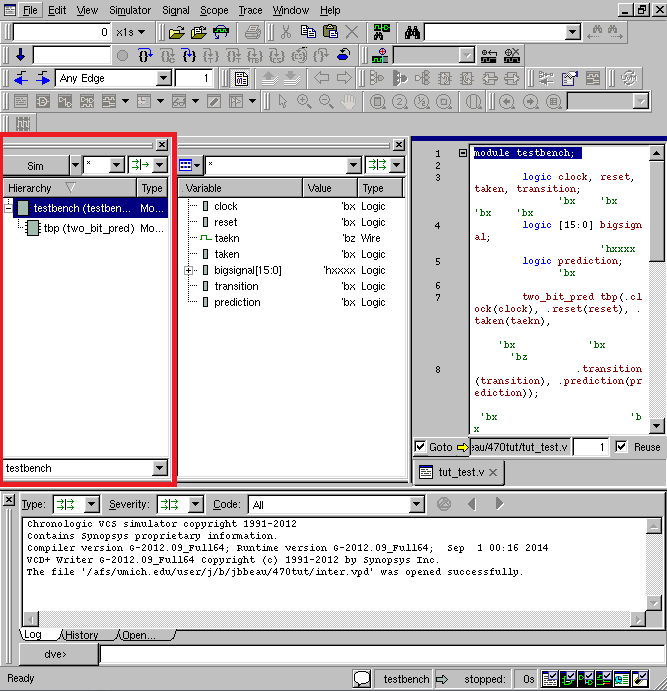
\includegraphics[scale=0.85]{mod-hier-pane}
        	\caption{The DVE Window with the Module Hierarchy Pane highlighted}
        	\label{fig:mod-hier-pane}
    	\end{center}
    \end{figure}


In \cref{fig:mod-hier-pane}, the pane on the far left of the DVE window is the 
Module Hierarchy Pane. It contains the names of the signals you might be 
interested in, grouped hierarchically by module. You will need this list to 
select signals you want to look at in other views and panes. 

In our tutorial, we have a testbench which instantiates another module. Expand
the testbench (click the plus icon to the left) in the pane to see the submodule. You'll notice that the submodule is called \texttt{tbp}, which is not the name of the \texttt{two\_bit\_pred}
module, but rather the name of the instantiation in the testbench. Make sure to use 
meaningful names for instantiations when you implement your own designs. 

\subsubsection{Data Pane}
\begin{figure}[H]
	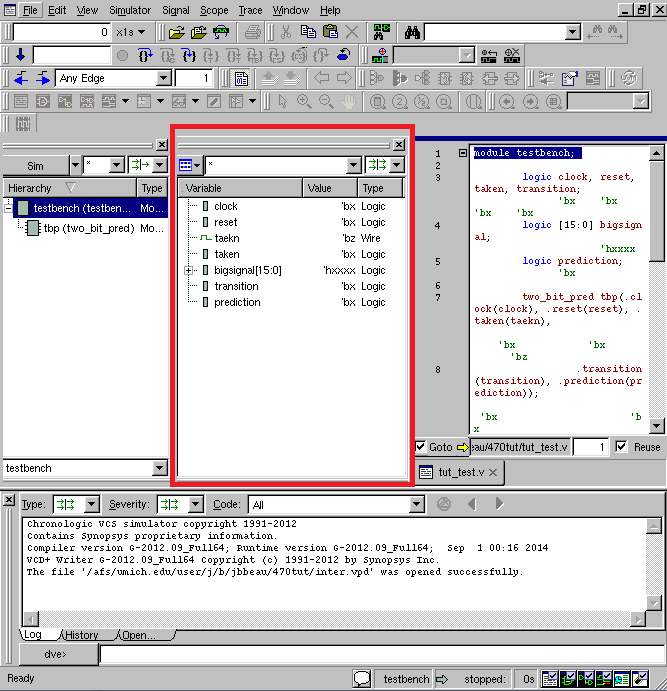
\includegraphics[width=\textwidth]{data-pane}
	\caption{The DVE Window with the Data Pane highlighted}
	\label{fig:data-pane}
\end{figure}

In \cref{fig:data-pane}, the data pane, located in the middle of the DVE window
is highlighted. This pane lists the signals in the currently selected module in
the module hierarchy pane. This is where you select the signals whose waveforms 
you would like to view. You can select multiple signals by holding down \keys{\shift}(shift) and clicking to select a group
or holding down \keys{\ctrl} and clicking to select multiple individual
signals. Select all the signals available in the testbench and right click on
the highlighted group, then go to \menu[,]{Add to waves,New wave view} to open the
waveform viewer. If, at some point later on, you need to add more signals to the
waveform viewer, you can do so by selecting them here and selecting 
\menu[,]{Add to waves,Add to [wave name]}.

\subsubsection{Waveform Viewer}
\begin{figure}[H]
	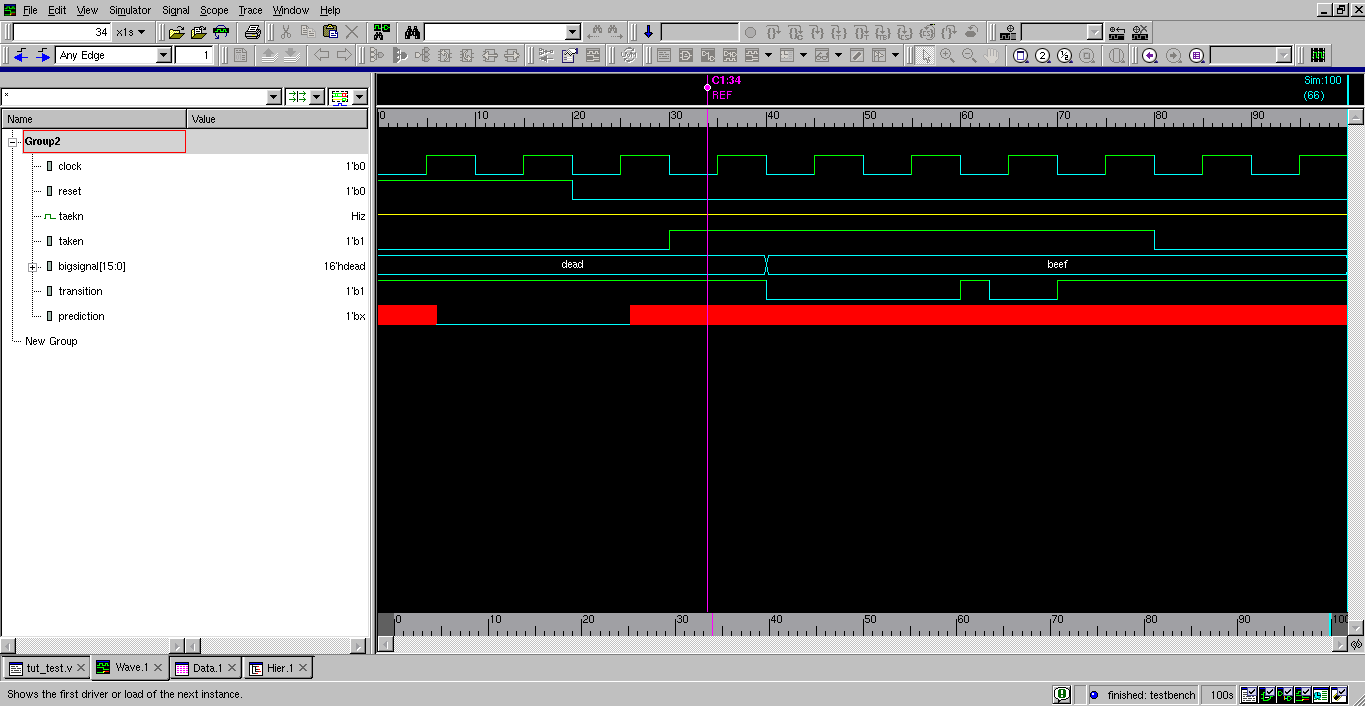
\includegraphics[width=\textwidth]{waveform-viewer}
	\caption{The Waveform Viewer Window}
	\label{fig:waveform}
\end{figure}

You will see a new window pop open, called the Waveform Viewer, which is shown
in \cref{fig:waveform}. In this new window, you need to go to
\menu[,]{Simulator,Start/continue} or press \keys{F5} to start the simulation and 
populate the waveform viewer. At this point, if you added additional signals to
this view, they would have no waveform, until you reran the simulator. This can
be done by \menu[,]{Simulator,Stop} then \menu[,]{Simulator,Start} or by
pressing \keys{F5} twice. 

The waveform viewer is intended to facilitate debugging by showing you how
several signals change in relation to one another over time. The pane on the
left hand side of this window lists the names of the signals currently being
displayed. The right hand pane shows the signals themselves. At the bottom of
this window there is a scroll bar which moves through time, when zoomed in to
see specific signal transitions. Move to the right to see how the signals in the
module change. Now, try zooming in and out, as well as getting all of time on
the screen at once by going to \menu[,]{View,Zoom} or clicking one of the 
magnifying glass buttons at the top. 

Signals in the waveform viewer can be displayed several different ways, largely
related to the 4 state logic used in Verilog. The ``good'' signals \texttt{0}
and \texttt{1} are shown as green signal lines with transitions between the two
values as appropriate. The ``bad'' signals \texttt{X} and \texttt{Z} show up as
a red block where the signal should be and a yellow line half way between
\texttt{0} and \texttt{1}, respectively. Both of these can be seen in the
provided module. Try to find them now. The signal \texttt{prediction} is an
example of the unknown value, \texttt{X}, after time 26, and the \texttt{taekn} 
signal is an example of the unconnected value, \texttt{Z}. These all apply to
1-bit signals. When we have a larger bus, values are displayed with their
hexadecimal value with marks where the value transitions. If any part of a bus
is \texttt{X}, it will show the whole thing as \texttt{X}, and similarly for
\texttt{Z}, it will show the hexadecimal value with the unconnected portions
marked with a \texttt{z}. If you would rather have buses display their value in
some other base, you can right click on the signal value in the left hand pane
and choose the \menu[,]{Radix} option. You can also expand the bus into all its
individual signals by clicking on the plus next to the signal name.

You can click on the waveform itself to drop a marker, which helps line up 
values across many signals at the same time. At the top of the waveform pane,
once you've placed a marker, there is a number corresponding to the time you've
set the marker at. Right clicking on this number gives you the option to advance
forward by an amount or to the next clock tick. 

Signals can be dragged around to group them more logically/helpfully. You can
also remove signals by highlighting them and then pressing the \keys{delete}
key.

\subsubsection{Source Pane}
\begin{figure}[H]
    \begin{center}
	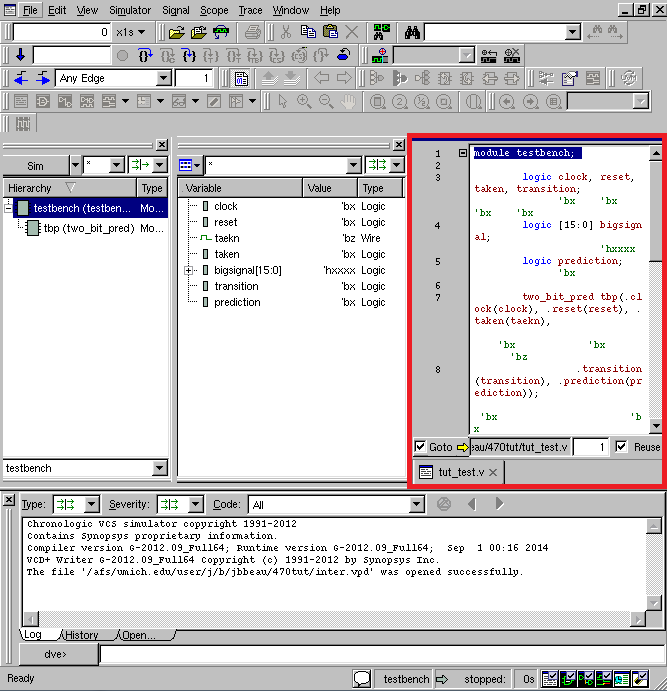
\includegraphics[scale=0.85]{source-pane}
	\caption{The DVE Window with the Source Pane highlighted}
	\label{fig:source-pane}
	\end{center}
\end{figure}

The source pane is on the right hand side of the DVE window, and is highlighted
in \cref{fig:source-pane}. It shows the Verilog source for the module you're
currently examining. This allows you to examine what exactly is generating a
signal. It can also let you double check that the file you've just edited to fix
a bug is the one you're now compiling/simulating. To change the file being
displayed, drag a module from the hierarchy pane over to see it. Similarly,
dragging a signal name over to the source pane to highlight its definition. To
view the current values of signals from the simulator in the source pane, right
click on the source pane and select \menu{Annotate Values}. You should now see
values next to each signal.


\subsubsection{Schematic Pane}
\begin{figure}[H]
	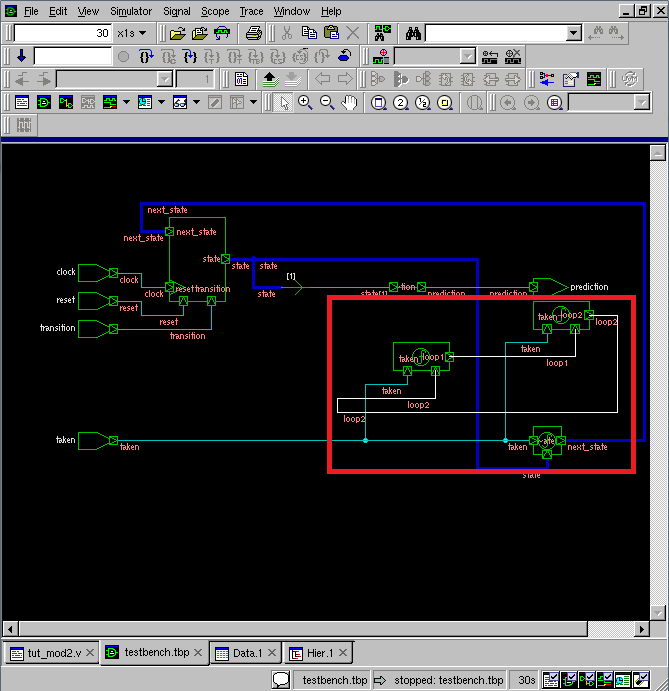
\includegraphics[width=\textwidth]{schematic-viewer}
	\caption{The Schematic Viewer}
	\label{fig:schematic-viewer}
\end{figure}

\Cref{fig:schematic-viewer} shows the schematic viewer. You can open up a 
schematic of any particular module by right clicking on it in the module 
hierarchy pane and selecting \menu{Show Schematic} from the menu. This can be 
useful in tracking where signals are coming from after synthesis. 

\subsubsection{Debugging Example}
Now that you've learned about many of the features of DVE, it's time to use it
to debug the module you've been given. 

The output of the \texttt{two\_bit\_pred} module is the \texttt{prediction}
signal. This signal goes to \texttt{X} at time 25 and stays there for the rest
of the simulation. Why would that happen? Let's figure it out.

For a signal to be unknown, one of its drivers must also be unknown, which if we
follow this logic down all the way means that one of the inputs somewhere is
unknown. So,we need to start by looking at how \texttt{prediction} gets set. The 
source for \texttt{tbp} should already be open, so let's use that to trace back 
to where the problem is. Let's also add the \texttt{tbp} module signals to the
waveform viewer so we can see the signals in that module. Looking at the source,
we can see that \texttt{prediction} is simply set equal to a bit of signal
\texttt{state}. Looking at the waveform viewer, we see that, as expected,
\texttt{state} is unknown at the same times. Now we want to check the signals 
that define \texttt{state}. We can see that \texttt{state} either takes on a 
known value of \texttt{01}, or it takes on the value of \texttt{next\_state}. 
So again, now we need to trace back to which values set \texttt{next\_state}.
Looking at this, we can see that \texttt{next\_state} is determined by
\texttt{state} and \texttt{taken}. We already know state is broken, so we need 
to look at \texttt{taken}. On the waveform viewer, we see that \texttt{taken}
always has a value of \texttt{Z}, unconnected. Because \texttt{taken} is an 
input into this module, we know the problem is in how the testbench is 
connecting to this module. Now let's drag the \texttt{testbench} module into the
source viewer so we can look for the problem. Looking at where \texttt{tbp} is 
instantiated, we can see that there was a typo. \texttt{.taken(taekn)} should 
have been \texttt{.taken(taken)} on line 7. The compiler assumed \texttt{taekn}
was just a wire not being driven and although it gave a warning, it did not give
a compiler error on this. These little bugs can often be very annoying to deal
with.

Now that we've found the bug, we want to save the waveform viewer configuration
so we can just easily reload them when we run the waveform viewer again. It may
not seem to be a big deal right now, but eventually when you're working with 
hundreds of signals, only a few of which are related to a problem you're trying
to debug, it can be very annoying to try to find and place them on the waveform
viewer every time. To do this, on the waveform viewer go to \menu[,]{File,Save
Session}. Type in a filename, like \texttt{view01.tcl} or, in the future, any 
name you want. It will be useful to keep the names descriptive as there may be 
different sets of signals to look at for different parts of a module you're 
testing. Now exit DVE.

Use your favorite text editor to fix that typo in \texttt{tut\_test.v}. When 
you're finished, type make clean and then \texttt{make dve} to recompile and 
reload the waveforms so we can double check that it's working properly now. Now 
on the DVE window, go to \menu[,]{File,Load Session}. Select your
\texttt{view01.tcl} file and press OK. The waveform viewer, complete with the 
original signals, should appear. Run the simulation again. Here we can see, that
everything is working properly now. 

Now, let's find another bug. Open up the provided \texttt{Makefile} and change
the value of the \texttt{SIMFILES} variable to \texttt{tut\_mod2.v} This module
has an infinite loop, which requires one more option in DVE. First, run
\texttt{make}, but when you've noticed that it hangs without printing anything,
kill the job with \keys{\ctrl + $\backslash$}. Now, run \texttt{make clean} to
remove the files the last command created and then run \texttt{make dve} to
start debugging the infinite loop.

The DVE window should appear. Now let’s find that infinite loop. Add the signals
to the waveform viewer. To find out where it is, run the simulator with the
\keys{F5} key. The waveform viewer should hang and a red dot in the toolbox 
above should get enabled. Now click on \menu[,]{Simulator,Terminate}. You can 
now see that the simulation was hung at time 25. The problem must be around here
somewhere. We are now at time 30. Now let’s find out where we’re looping. Click
on \menu[,]{Simulator,Step/Next,Next} a few times and look at the tbp source 
code. We seem to be going between \texttt{tut\_mod2.v:11} and
\texttt{tut\_mod2.v:12}. That means that lines 11 and 12 of \texttt{tut\_mod2.v}
are causing the problem. We now know that the problem is in our module (not our 
testbench). In the tbp source, right click and select \menu{Annotate Values} to 
monitor the values of each wire. We want to see how we got to this state. If we 
look at the source window, we can see that lines 11 and 12 are assignments to 
\texttt{loop1} and \texttt{loop2}. If we click next a few times and watch the 
values, we can see that both \texttt{loop1} and \texttt{loop2} keep changing 
even though no time is actually passing. This is a sure sign of circular logic.
Since \texttt{loop1} is dependent on \texttt{loop2}, and \texttt{loop2} is 
dependent on \texttt{loop1}, the circular path is fairly obvious in this case. 
We now have enough information to fix the bug, but in this example, there’s
nothing to really fix, since the \texttt{loop1} and \texttt{loop2} variables are
not used for anything, so we can just leave the design alone and finish up. 

This concludes our introduction to DVE, but there are a number of other useful 
features in the waveform viewer. Feel free to explore and try other things on 
your own.

\subsection{The Synthesis Tool: \texttt{dc\_shell}}
In this class we require that your hardware designs really represent hardware
and we judge your final project on the overall speed of your design. To 
 accomplish this you will need to synthesize your design. The synthesis tool
attempts to create an actual circuit level implementation of your Verilog design
description. This circuit level design is actually a Verilog file itself, but it
is structural Verilog and uses a library of standard cells that another tool can
lay out on a real chip. One benefit of the output being a Verilog file is that 
we can simulate the circuit level design in the same way we simulate your 
behavioral design. Thus, we can test your synthesized design and if it does not
behave properly your design is not considered to be synthesizable and is 
therefore incorrect (though we do give partial credit).The clock speed of the 
circuit that it generates will be the clock speed we use for your design. We 
won’t go into great detail about synthesis in this tutorial but we will show you
the basic commands. We provide greater depth in Lab 2.

We interact with the synthesis tool, Synopsys Design Compiler, through a script
of options and commands written in the Tool Control Language, which is
abbreviated TCL (\texttt{*.tcl}) and spoken like the word ``tickle.'' We have
provided you with a synthesis script called \texttt{tut\_synth.tcl}, which is
run by a Make rule, shown in \cref{fig:make-syn}. Open the script in the editor
of your choice. Read through it, the commands are actually pretty intuitively
named, though some of them are a bit confusing. We will explain more of this to
you later, but the part you need to be familiar with now is marked with a
comment saying ``\texttt{The following five lines must be updated for every new
design}.'' The first line of this section tells the tool what Verilog design
files to read. The second line tells the tool the name of your toplevel module.
The third line names the clock signal, and the fourth line sets the clock period. A higher clock period will yield faster synthesis times, while a lower
one will take longer because it requires more effort on the part of the
synthesis tool. A clock period set too small may not even be possible. We will
explore this design constraint in Project 2.

\begin{figure}[H]
	\begin{minted}[frame=lines,obeytabs,tabsize=4]{makefile}
two_bit_pred.vg:	tut_mod.v tut_synth.tcl
	dc_shell-t -f tut_synth.tcl | tee synth.out
	\end{minted}
	\caption{The synthesis Make rule.}
	\label{fig:make-syn}
\end{figure}

You will need to add the Make rule from \cref{fig:make-syn} to your
\texttt{Makefile}. \textbf{Do not simply copy-paste it, retype it}. Make is very
persnickety about whitespace, so make sure you put a single tab after the rule
name (after the colon on the first line) and another single tab at the beginning
of the second line. Once you have the rule added and the correct names in
\texttt{tut\_synth.tcl}, run \texttt{make syn} to synthesize and simulate the
synthesized design.

This will produce four files. Please open them and read them. 

\begin{enumerate}
	\item \texttt{two\_bit\_pred.chk} -- This file contains errors if something
		went wrong, otherwise it will be empty (or occasionally contains a single number; you can ignore that).
	\item \texttt{two\_bit\_pred.ddc} -- This file contains the proprietary
		Synopsys representation of the synthesized design. It can be included
		like a Verilog design file in synthesis, either to be optimized again or
		as a black box.
	\item \texttt{two\_bit\_pred.rep} -- This file contains the timing report
		for your design. We will cover it in greater detail in Lab 2.
	\item \texttt{two\_bit\_pred.vg} -- This file contains the structural
		Verilog that the synthesis tool generated for your design and design
		constraints.
\end{enumerate}

\section{Assignment}
You will now write and debug a design from scratch, though you probably want to
use designs we've shown you as templates.

\subsection{Design}
\begin{figure}[H]
	\centering
	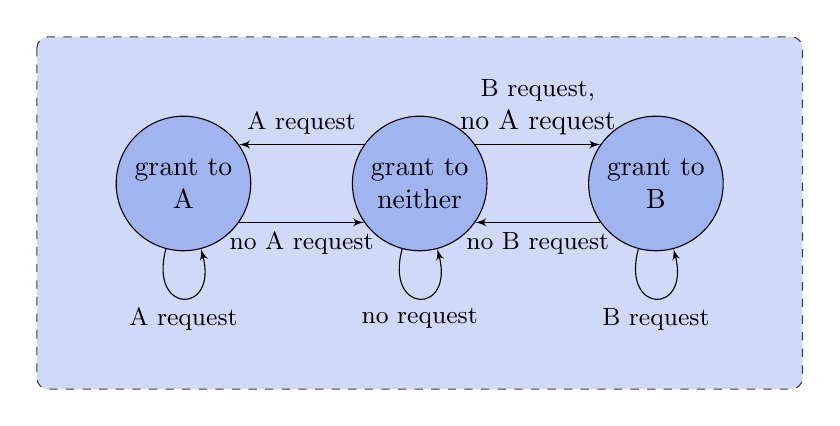
\begin{tikzpicture}[auto, node distance=3cm,>=latex',every text node
		part/.style={align=center}]
		\def\blockdist{2em}
		\def\edgedist{2em}

		\begin{pgfonlayer}{foreground}
			\node[state] (center) {grant to \\ neither};
			\node[state,left of=center] (left) {grant to \\ A};
			\node[state,right of=center] (right) {grant to \\ B};

			\draw[->] (center.145) -- node[pos=0.5,anchor=south] {\small A request}
			(left.35);
			\draw[->] (left.325) -- node[pos=0.5,anchor=north] {\small no A request}
			(center.215);
			\draw[->] (center.35) -- node[pos=0.5,anchor=south] {\small B request, \\ no
			A request} (right.145);
			\draw[->] (right.215) -- node[pos=0.5,anchor=north] {\small no B
			request} (center.325);

			\draw[->] (center) to[out=255,in=285,looseness=5]
			node[pos=0.5,anchor=north] {\small no request} (center);
			\draw[->] (left) to[out=255,in=285,looseness=5]
			node[pos=0.5,anchor=north] {\small A request} (left);
			\draw[->] (right) to[out=255,in=285,looseness=5]
			node[pos=0.5,anchor=north] {\small B request} (right);
		\end{pgfonlayer}
		\begin{pgfonlayer}{background}
			\path (center.north -| left.west)+(-1,1.0) node (a) {};
			\path (right.east |- right.south)+(1,-1.75) node (b) {};
			\path[fill=RoyalBlue!25, rounded corners, draw=black!75, dashed] (a) rectangle (b);
		\end{pgfonlayer}
	\end{tikzpicture}
	
	\caption{This is a Moore state machine for an arbiter, which conceptually 
		would be connected to two requesters, A and B, at some higher level, and
		should provide signals to each indicating whether control has been 
		granted to it.} 
	\label{fig:state}
\end{figure}

Begin by examining the state machine in \cref{fig:state}. What are the inputs
and the outputs? What state needs to be stored, and given this, what registers
do you need? What does the combinational logic look like?

\subsection{Implementation}
The Verilog you write to implement the state machine above should be put into a
file called \texttt{arbiter.v}. You will also need a testbench,
\texttt{arbiter\_test.v}, to test the module. Ideally you should try to write a
testbench that produces the correct output for the module to test against, but
for this lab that is not vital. 

\subsection{Testing}
Compile, run and debug your design using the tools and techniques described
above. Note that you will need to modify the \texttt{Makefile}. 

\subsection{Synthesize}
Modify the \texttt{synth.tcl} provided with this lab to synthesize the module
you've just written. Synthesize the module. Verify that it synthesized
correctly.

\section{Submission}
You must prove your testbench thoroughly tests your behavioral and structural verilog using either DVE or GTKwave. Place yourself on the \href{https://oh.eecs.umich.edu/courses/eecs470}{\underline{help queue}} during office hours once you're confident you've completed the lab satisfactorily. The assignment is due by the end of next week's lab.

% Once you're done with the assignment, you will need to submit it. To do this,
% you will run the following command:

% \noindent
% \texttt{\$ /afs/umich.edu/user/w/c/wcunning/Public/470submit -l1 lab1}

\end{document}